\documentclass{article}
\usepackage[utf8]{inputenc}
\usepackage[version=3]{mhchem}
\usepackage{graphicx}
\usepackage{float}
\usepackage[dvipsnames]{xcolor}
\usepackage[table,xcdraw]{xcolor}
\usepackage{indentfirst} 
\usepackage{float}
\restylefloat{table}
\usepackage{adjustbox}
\usepackage{hyperref}
\usepackage{blindtext}
\usepackage{fancyhdr}
\usepackage{titlepic}
\pagestyle{fancy}
\fancyhf{}

\pagestyle{plain} 
\usepackage{xcolor}\usepackage{listings}\usepackage[UKenglish]{babel}\usepackage{amsmath}\usepackage{braket}\usepackage{physics}\usepackage{booktabs}


%---------------------------------
\title{TQ-Using IBM Open-Quantum-Computing Services to test Violation of
Local Realism with Mermin Inequalities}


\author{
Gonçalo Gouveia\\
  \texttt{2018277419|MEF}\\
  uc2018277419@student.uc.pt\\
  \\
}


\begin{document}
\maketitle

\thispagestyle{empty}
\clearpage
\pagebreak
\section{}
\subsection*{a)}


Testing the inequalities for the $M_{3}$ polynomial:
\begin{equation}
  M_{3}=a_{1} a_{2} a_{3}^{\prime}+a_{1} a_{2}^{\prime} a_{3}+a_{1}^{\prime} a_{2} a_{3}-a_{1}^{\prime} a_{2}^{\prime} a_{3}^{\prime}  
\end{equation}

Where $a_{i}$ and $a_{i}^{\prime}$ will be Pauli operators.The maximum value $\left\langle M_{3}\right\rangle$ can take for 3-qubits is $2^{n-1}=2^{3-1}=4$\textcolor{blue}{[3]}.\\


$\left\langle M_{3}\right\rangle$ is maximized by the GHZ-like states \textcolor{blue}{[2]}:
$$
|\Phi\rangle_{G H Z}=\frac{1}{\sqrt{2}}\left(|000\rangle+e^{i \phi}|111\rangle\right)
$$
Where $\phi$ is a relative phase factor which will depend on our choice for the $a_{i}$ and $a_{i}^{\prime}$. For $a_{i}=\sigma_{x}$ and $a_{i}^{\prime}=\sigma_{y}, \phi=\pi / 2$. For $a_{i}^{\prime}=\sigma_{x}$ and $a_{i}=\sigma_{y}, \phi=\pi$, $|\Phi\rangle_{G H Z}$ maximizes $\left\langle M_{3}\right\rangle$. If we take $\phi=\pi / 2$,  becomes:
\begin{equation}
\sigma_{x}^{1} \sigma_{x}^{2} \sigma_{y}^{3}+\sigma_{x}^{1} \sigma_{y}^{2} \sigma_{x}^{3}+\sigma_{y}^{1} \sigma_{x}^{2} \sigma_{x}^{3}-\sigma_{y}^{1} \sigma_{y}^{2} \sigma_{y}^{3}
\end{equation}
Therefore:

\begin{equation*}
    \sigma^1_x\sigma^2_x\sigma^3_y(\ket{000}+i\ket{111})=\ket{000}+i\ket{111}=\sqrt{2}\ket{\phi_{GHZ}}
\end{equation*}
\begin{equation*}
     \sigma^1_x\sigma^2_y\sigma^3_x(\ket{000}+i\ket{111})=\ket{000}+i\ket{111} =\sqrt{2}\ket{\phi_{GHZ}}  
\end{equation*}
\begin{equation*}
     \sigma^1_y\sigma^2_x\sigma^3_x(\ket{000}+i\ket{111})=\ket{000}+i\ket{111}=\sqrt{2}\ket{\phi_{GHZ}}   
\end{equation*}
\begin{equation*}
     -\sigma^1_y\sigma^2_y\sigma^3_y(\ket{000}+i\ket{111})=\ket{000}+i\ket{111}=\sqrt{2}\ket{\phi_{GHZ}}   
\end{equation*}
Therefore, summing all of the above, we get


\begin{equation*}
    M_3\ket{\phi}=4\ket{\phi_{GHZ}}\\
\end{equation*}
\begin{equation*}
    \braket{\phi_{GHZ}}=\frac{1}{2}(\bra{000}-i\bra{111})(\ket{000}i\ket{111})=1
\end{equation*}
Thus,
\begin{equation*}
    \bra{\phi_{GHZ}}M_3\ket{\phi_{GHZ}}=4\bra{\phi_{GHZ}}\ket{\phi_{GHZ}}=4
\end{equation*}
\pagebreak

Proceeding the same way from $\phi=\pi$. In this case:

\begin{equation}
\sigma_{y}^{1} \sigma_{y}^{2} \sigma_{x}^{3}+\sigma_{y}^{1} \sigma_{x}^{2} \sigma_{y}^{3}+\sigma_{x}^{1} \sigma_{y}^{2} \sigma_{y}^{3}-\sigma_{x}^{1} \sigma_{x}^{2} \sigma_{x}^{3}
\end{equation}
Therefore:

\begin{equation*}
    \sigma^1_y\sigma^2_y\sigma^3_x(\ket{000}-\ket{111})=\ket{000}-\ket{111}
\end{equation*}
\begin{equation*}
     \sigma^1_y\sigma^2_x\sigma^3_y(\ket{000}-\ket{111})=\ket{000}-\ket{111}   
\end{equation*}
\begin{equation*}
     \sigma^1_y\sigma^2_y\sigma^3_x(\ket{000}-\ket{111})=\ket{000}-\ket{111}
\end{equation*}
\begin{equation*}
     -\sigma^1_x\sigma^2_x\sigma^3_x(\ket{000}-\ket{111})=\ket{000}-\ket{111}  
\end{equation*}
Similarly, to before:
\begin{equation*}
    \bra{\phi_{GHZ}}M_3\ket{\phi_{GHZ}}=4\bra{\phi_{GHZ}}\ket{\phi_{GHZ}}=4
\end{equation*}
And again, summing all of the above, we get:
$$
\left\langle M_{3}\right\rangle_{G H Z}=4\left\langle\Phi_{G H Z} \mid \Phi_{G H Z}\right\rangle=4
$$
Which proves that the GHZ-like states maximize $\left\langle M_{3}\right\rangle$.


\subsection*{b)}
For the 3 Qubit case. Assuming $a_i=\sigma_x$, $a'_i=\sigma_y$, making $ \phi=\pi$.      
This GHZ state can be simulated with
the following simple circuit:
\begin{figure} [H]
    \centering
    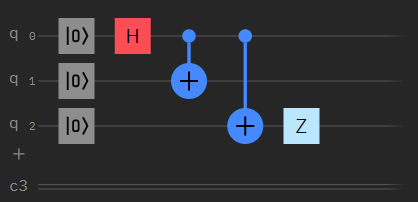
\includegraphics[scale = 0.75]{1.png}
    \caption{Circuit for the GHZ State simulation}
    \label{fig:my_label}
\end{figure}
\begin{figure} [H]
    \centering
    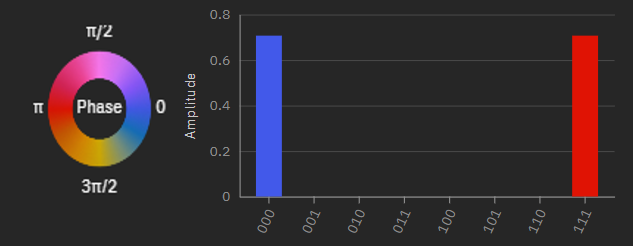
\includegraphics[scale = 0.65]{3.png}
    \caption{Computational basis states.}
    \label{fig:my_label}
\end{figure}

The final $\boxed{Z}$ gate on $q_{3}$ will give the state the desired $\phi$ phase.\\

However, since our computer is far from the theoretical idealism, we should pick only one of the qubits to be target of the CNOT operation. Thus, one does use the equivalence that $\mathrm{CNOT}_{1 \rightarrow 2}=$ $\left(H_{1} \otimes H_{2}\right) \mathrm{CNOT}_{2 \rightarrow 1}\left(H_{1} \otimes H_{2}\right)$ . In adiction, the phase gate $\boxed{Z}$ can be put
anywhere, we  place it in the most robust qubit, that is,
the one with less gates.\textcolor{blue}{[1]}
\begin{figure} [H]
    \centering
    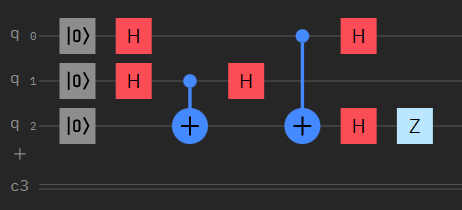
\includegraphics[scale = 0.8]{2.png}
    \caption{Used circuit for the GHZ State simulation}
    \label{fig:my_label}
\end{figure}
\begin{figure} [H]
    \centering
    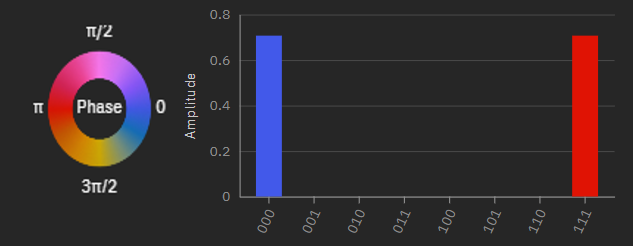
\includegraphics[scale = 0.6]{3.png}
    \caption{Computational basis states.}
\end{figure}
Acting accordingly to the problem we want to measure, Before each measurement $q_{i}$ in $\mathrm{x}$-basis, we put an Hadamard gate followed by a z-basis measurement in that qubit channel. If we want to measure in the y-basis, we apply a $S^{\dagger}$ and one follows as mentioned before.\\

The following circuits were ran 1024 times, not overloading the quantum computers with non research focused simulations, which yield in obtaining the following data:




% \usepackage{booktabs}

\begin{figure} [H]
    \centering
    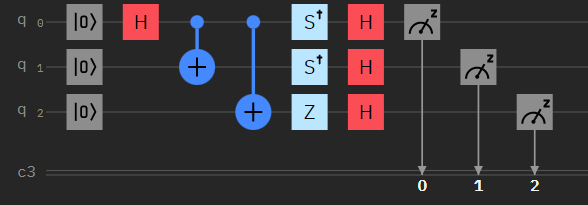
\includegraphics[scale = 0.85]{YYXIdeal.png}
    \caption{YYX ideal circuit.}
    \label{fig:my_label}
\end{figure}
Counts for each result are expressed in probabilities
computed out of 1024 runs.


\begin{table}[H]
\centering
\begin{tabular}{@{}llllllllll@{}}
\toprule
State       & \ket{111} & \ket{110}   & \ket{101} & \ket{100} & \ket{011} & \ket{010}  & \ket{001} & \ket{000}  \\ \midrule
Eigenvalue  & -1 &1  & 1  & -1 & 1 & -1 & -1 & 1 \\ \midrule
Probability & 0.015 & 0.193 & 0.198 & 0.023 & 0.225 & 0.038 & 0.055 & 0.250 \\ \bottomrule
\end{tabular}
\end{table}
\begin{equation*}
 \left\langle\sigma_{y}^{1} \sigma_{y}^{2} \sigma_{x}^{3}\right\rangle_{\text {Perfect }}=0.74 \pm 0.02
 \end{equation*}\\
 
Noticing that we only need to simulate 2 circuits, since the cross terms of (3) yield the same probabilities \textcolor{blue}{[1]}.
 \begin{equation*}
      \left\langle\sigma_{y}^{1} \sigma_{y}^{2} \sigma_{x}^{3}\right\rangle_{\text {Perfect }}= \left\langle\sigma_{y}^{1} \sigma_{x}^{2} \sigma_{y}^{3}\right\rangle_{\text {Perfect }}= \left\langle\sigma_{x}^{1} \sigma_{y}^{2} \sigma_{y}^{3}\right\rangle_{\text {Perfect }}
 \end{equation*}
 
 
 \\
 Every uncertainty was calculated assuming the probabilities follow a multinomial distribution: $\delta_{p}=\sqrt{p(1-p) / N}$. \textcolor{blue}{[1]}
 
\begin{figure} [H]
    \centering
    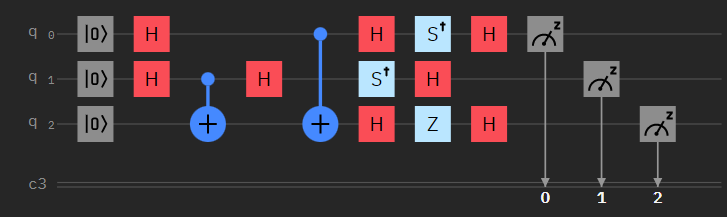
\includegraphics[scale = 0.7]{YYXIReal.png}
    \caption{YYX measurement circuit.}
    \label{fig:my_label}
\end{figure}

\begin{table}[H]
\centering
\begin{tabular}{@{}llllllllll@{}}
\toprule
State       & \ket{111} & \ket{110}  & \ket{101} & \ket{100} & \ket{011} & \ket{010}  & \ket{001} & \ket{000}  \\ \midrule
Eigenvalue  &  -1 &1  & 1  & -1 & 1 & -1 & -1 & 1\\ \midrule
Probability &0.033  & 0.164 & 0.173&0.046  & 0.2025 & 0.052 & 0.106 & 0.217 \\ \bottomrule
\end{tabular}
\end{table}
\begin{equation*}
 \left\langle\sigma_{y}^{1} \sigma_{y}^{2} \sigma_{x}^{3}\right\rangle=0.52 \pm 0.02
 \end{equation*}
 
 \begin{equation*}
      \left\langle\sigma_{y}^{1} \sigma_{y}^{2} \sigma_{x}^{3}\right\rangle= \left\langle\sigma_{y}^{1} \sigma_{x}^{2} \sigma_{y}^{3}\right\rangle= \left\langle\sigma_{x}^{1} \sigma_{y}^{2} \sigma_{y}^{3}\right\rangle
 \end{equation*}


\begin{figure} [H]
    \centering
    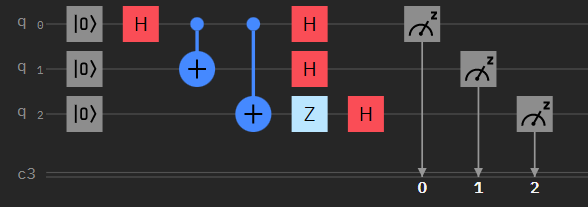
\includegraphics[scale = 0.8]{XXXideal.png}
    \caption{XXX ideal circuit.}
\end{figure}






\begin{table}[H]
\centering
\begin{tabular}{@{}llllllllll@{}}
\toprule
State       & \ket{111} & \ket{110}  &  \ket{101} & \ket{100} & \ket{011} & \ket{010}  & \ket{001} & \ket{000}  \\ \midrule
Eigenvalue  &   -1 &1  & 1  & -1 & 1 & -1 & -1 & 1 \\ \midrule
Probability & 0.1845 & 0.0254 & 0.0264 & 0.254 & 0.024 & 0.177  & 0.250  & 0.056 \\ \bottomrule
\end{tabular}
\end{table}
\begin{equation*}
 \left\langle\sigma_{x}^{1} \sigma_{x}^{2} \sigma_{x}^{3}\right\rangle_{ideal}=-0.73 \pm 0.02
 \end{equation*}

\begin{figure} [H]
    \centering
    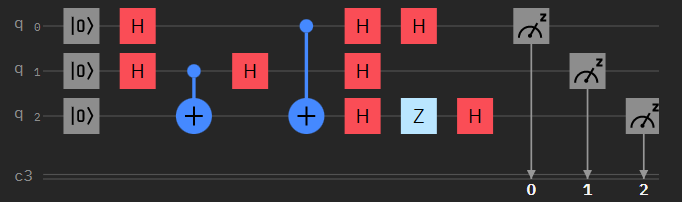
\includegraphics[scale = 0.7]{XXXreal.png}
    \caption{XXX measurement circuit.}
    \label{fig:my_label}
\end{figure}

\begin{table}[H]
\centering
\begin{tabular}{@{}llllllllll@{}}
\toprule
State       & \ket{111} & \ket{110}   & \ket{101} & \ket{100} & \ket{011} & \ket{010}  & \ket{001} & \ket{000}  \\ \midrule
Eigenvalue  &   -1 &1  & 1  & -1 & 1 & -1 & -1 & 1 \\ \midrule
Probability & 0.178 & 0.015 & 0.043 & 0.2543 & 0.019 & 0.188 & 0.240 &  0.068  \\ \bottomrule
\end{tabular}
\end{table}

\begin{equation*}
 \left\langle\sigma_{x}^{1} \sigma_{x}^{2} \sigma_{x}^{3}\right\rangle=-0.71 \pm 0.02
 \end{equation*}
\\

\section{Results \& Discussion}

 According to \textcolor{blue}{[1]}
:
\begin{equation*}
\left\langle M_{3}\right\rangle_{G H Z}=\sigma_{y}^{1} \sigma_{y}^{2} \sigma_{x}^{3}+\sigma_{y}^{1} \sigma_{x}^{2} \sigma_{y}^{3}+\sigma_{x}^{1} \sigma_{y}^{2} \sigma_{y}^{3}-\sigma_{x}^{1} \sigma_{x}^{2} \sigma_{x}^{3}
\end{equation*}

Noticing again that the first 3 terms do yield the same probabilities.

$$
\left\langle M_{3}\right\rangle_{G H Z}=3\left\langle\sigma_{y}^{1} \sigma_{y}^{2} \sigma_{x}^{3}\right\rangle-\sigma_{x}^{1} \sigma_{x}^{2} \sigma_{x}^{3}
$$\\

We obtain the final results of :
\begin{equation*}
    \left\langle M_{3}\right\rangle_{ideal}=2.95 \pm 0.06
\end{equation*}
\begin{equation*}
    \left\langle M_{3}\right\rangle=2.27 \pm 0.06
\end{equation*}


Which violate the Mermin Inequality for local realism $\left\langle M_{3}\right\rangle_{LR}\leq2.0$. \\
The difference between $\left\langle M_{3}\right\rangle_{ideal}$ and $ \left\langle M_{3}\right\rangle$ are mostly due to statistical fluctuations and 
gate errors. Mostly due to the CNOT gate errors, Both teh $\boxed{Z}$ and $\boxed{H}$ gates can be described with CNOT gates\\
This circuits were implemented in the IBM quantum computer in the system \emph{ibmq\_manila}, that at the given moment of the runs were with the following characteristics:


\begin{figure}[H]
    \centering
    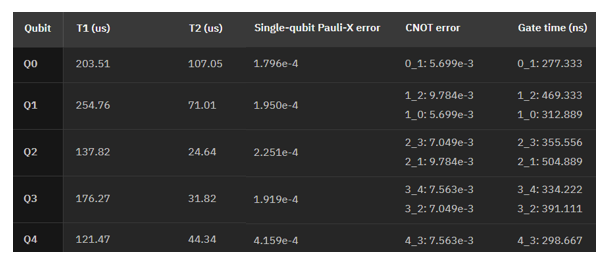
\includegraphics[scale = 0.6]{errrrrr.png}
    \caption{Calibration data in \emph{ibmq \_ manila}}
\end{figure}





\begin{thebibliography}{10}
\bibitem{Robotics}  
 Alsina, D. & Latorre, J. I. 2016, Phys. Rev. A, 94, 012314
\bibitem{Robotics} 
 Greenberger, D. M., Horne, M. A., & Zeilinger, A. 2007 [arXiv:0712.0921]

\bibitem{Robotics} 
Mermin, N. D. 1990, Phys. Rev. Lett., 65, 1838


\end{thebibliography}




\end{document}
